\documentclass[border=4pt,varwidth=17cm]{standalone}
\usepackage{amsmath,amssymb,mathrsfs,mathtools}
\usepackage{tikz}
\usetikzlibrary{positioning,fit,backgrounds,arrows.meta}
\def\RR{{\mathbb R}}\def\eps{\varepsilon}\def\then{\Rightarrow}
\def\J{\mathcal{J}_L}\def\A{\mathcal{A}_{f,g}}\def\Sol{\mathcal{S}_{f,g}}
\def\limsup{\mathop{\overline{\lim}}}\def\liminf{\mathop{\underline{\lim}}}
\def\Of{{\sf (O$_f$)}}\def\Og{{\sf (O$_g$)}}
\def\Rv{{\sf (R$_{\rm v}$)}}\def\Rh{{\sf (R$_{\rm h}$)}}
\begin{document}


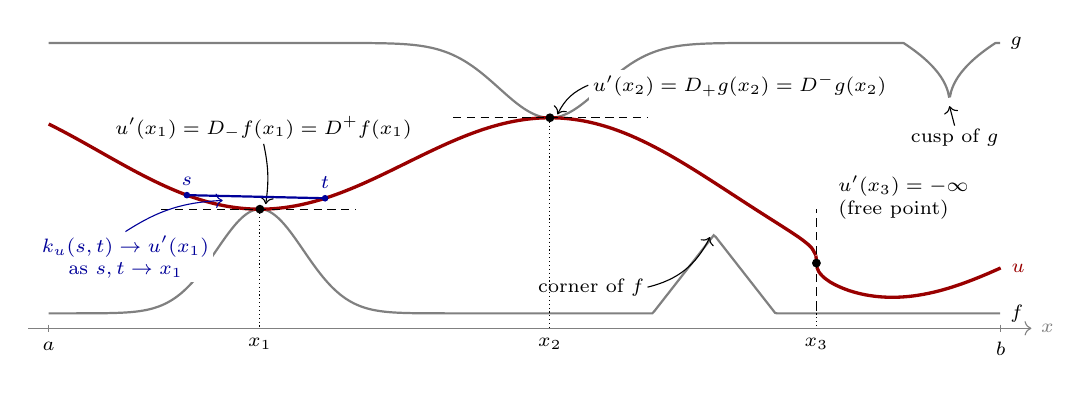
\begin{tikzpicture}[x=1.3cm, y=0.95cm, font=\scriptsize,
  declare function={S(\t)=-0.45*((\t<8) ? -1 : 1)*abs(\t-8)^(1/3);
    U(\t)=1.5+0.7*sin(deg(pi*(\t-4)/3))+S(\t);
    F(\t)=0.2+(1.5928-0.2)*exp(-((\t-2.5633)/0.6)^2);
    G(\t)=3.815-exp(-((\t-5.3965)/0.7)^2);
    FC(\t)=F(\t)+1.05*max(0,1-abs(\t-7)/0.6);
    GC(\t)=G(\t)-0.8*max(0,1-sqrt(abs(\t-9.3)/0.45));}]
  % axis and endpoints
  \draw[->, gray] (0.3,0) -- (10.1,0) node[right] {$x$};
  \draw[gray] (0.5,0.05) -- (0.5,-0.05) node[below, black] {$a$};
  \draw[gray] (9.8,0.05) -- (9.8,-0.05) node[below, black] {$b$};
  % obstacles
  \draw[thick, gray, domain=0.5:9.8, samples=466] plot (\x, {FC(\x)}) node[right, black] {$f$};
  \draw[thick, gray, domain=0.5:9.8, samples=931] plot (\x, {GC(\x)}) node[right, black] {$g$};
  % corners of the obstacles, away from the contact set
  \node[anchor=east, align=right, fill=white, inner sep=1pt] (cf) at (6.35,0.55) {corner of $f$};
  \draw[->, thin] (cf.east) to[bend right=25] (6.96,1.22);
  \node[align=center, fill=white, inner sep=1pt] (cg) at (9.35,2.55) {cusp of $g$};
  \draw[->, thin] (cg.north) -- (9.3,2.97);
  % solution
  \draw[very thick, red!60!black, domain=0.5:7.995, samples=200, smooth] plot (\x, {U(\x)});
  \draw[very thick, red!60!black, domain=8.005:9.8, samples=100, smooth] plot (\x, {U(\x)}) node[right] {$u$};
  \draw[very thick, red!60!black] (7.995,{U(7.995)}) -- (8.005,{U(8.005)});
  % contact with f
  \fill (2.5633,1.5928) circle (1.6pt);
  \draw[densely dashed] (1.6,1.5928) -- (3.5,1.5928);
  \draw[densely dotted] (2.5633,1.5928) -- (2.5633,0) node[below] {$x_1$};
  \node[align=center, fill=white, inner sep=1.5pt] (n1) at (2.6,2.68) {$u^\prime(x_1)=D_-f(x_1)=D^+f(x_1)$};
  \draw[->, thin] (n1.south) to[bend left=10] (2.62,1.66);
  % contact with g
  \fill (5.3965,2.81495) circle (1.6pt);
  \draw[densely dashed] (4.45,2.81495) -- (6.35,2.81495);
  \draw[densely dotted] (5.3965,2.81495) -- (5.3965,0) node[below] {$x_2$};
  \node[align=center, fill=white, inner sep=1.5pt] (n2) at (7.25,3.25) {$u^\prime(x_2)=D_+g(x_2)=D^-g(x_2)$};
  \draw[->, thin] (n2.west) to[bend right=20] (5.47,2.86);
  % singular free point
  \fill (8,{U(8.0001)}) circle (1.6pt);
  \draw[densely dashed] (8,0.25) -- (8,1.6);
  \draw[densely dotted] (8,0.25) -- (8,0) node[below] {$x_3$};
  \node[align=left, anchor=west] at (8.12,1.75) {$u^\prime(x_3)=-\infty$\\(free point)};
  % chord illustrating strict differentiability
  \draw[thick, blue!60!black] (1.85,{U(1.85)}) -- (3.2,{U(3.2)});
  \fill[blue!60!black] (1.85,{U(1.85)}) circle (1.2pt) node[above] {$s$} (3.2,{U(3.2)}) circle (1.2pt) node[above] {$t$};
  \node[blue!60!black, align=center, fill=white, inner sep=1.5pt] (nk) at (1.25,0.95) {$k_u(s,t)\to u^\prime(x_1)$\\ as $s,t\to x_1$};
  \draw[->, thin, blue!60!black] (nk.north) to[bend left=15] (2.2,{(U(1.85)+U(3.2))/2-0.05});
\end{tikzpicture}


\end{document}
